\clearpage
\chapter{Results}\label{chap:results}

\section{Overview}

Over 1 billion games were simulated in the process of evaluating the chromosomes
in this experiment. One thousand generations were evolved for every combination
of chromosome type (RGA, SGA, and TGA), population size (32, 128, 512, and
1024), number of games played by each chromosome per generation (7, 25, 50,
100), and fitness evaluator (FINISH\_ORDER (FO), NET\_WORTH (NetW),
NUM\_MONOPOLIES (NM), NUM\_PROPERTIES (NP), NUM\_WINS (NW), and TOURNAMENT
(TO)\footnote{For the tournament fitness evaluator the number of games was
determined by the population size and was not independent. So for TOURNAMENT,
1000 generations were evolved for every combination of population size and
chromosome type}). In this chapter, those four features are used to identify the
different populations: for example, RGA-512-50-NP refers the to RGA chromosome
population of size 512, where each player played 50 games per generation and the
fitness evaluator was NUM\_PROPERTIES. Results of the evolutionary process are
presented in the first section of this Chapter.

Results for the RGA chromosome are presented first, and in a large amount
detail. We also look briefly at the results for the SGA chromosomes, even though
players with this chromosome tended to evolve poorly. This is most likely due to
the fact that the data structure used for the SGA chromosomes is not well suited
to the problem domain. Finally, results for the TGA chromosomes are very briefly
discussed, but these players were essentially identical to the RGA chromosomes
and so do not provide any additional insight.

After the evolutionary process was complete, the best players from each
generation were competed in various combinations to validate the results. The
validation process is listed below. Because the evolution of SGA and TGA
chromosomes do not provide any useful information, the validation of the evolved
players focuses exclusively on results obtained from the RGA chromosomes.

\begin{enumerate} 
  \item {Intra-population validation}
  \begin{enumerate}
    \item {For each RGA population select the best player from generation 250,
    500, 750, and 999}
    \item {Compete the 4 players in 100 games}
    \item {Record the fitness scores for FINISH\_ORDER and NUM\_WINS}
    \item {Repeat 50 times with evolution}
    \item {Use Student's t-test to compare average fitness}
  \end{enumerate}
  \item {Inter-population validation for fitness evaluator}
  \begin{enumerate} 
    \item {From generation 999 of a set of populations differing only by
    original fitness evaluator, select the best player under each fitness
    evaluator (results in 6 players)} 
    \item {Compete the 6 players in 50 games}
    \item {Record the fitness scores for FINISH\_ORDER}
    \item {Repeat 30 times}
    \item {Use Student's t-test to compare average fitness}
  \end {enumerate}
  \item {Real-world validation 1}
  \begin{enumerate} 
    \item {Select the top 4 players from generations 250, 500, 750, and 999 from
    the RGA-1024-100-FO population}
    \item {compete the players randomly against human players}
    \item {Record the fitness scores for FINISH\_ORDER}
    \item {Compare average fitness and average net worth among all players}
  \end {enumerate}
  \item {Real-world validation 2}
  \begin{enumerate} 
    \item {Select the top 4 players from generation 999 from the RGA-1024-100-FO 
    population}
    \item {Compete the players randomly against human players using an updated 
    property trading algorithm}
    \item {Record the fitness scores for FINISH\_ORDER}
    \item {Compare average fitness and average net worth among all players}
  \end {enumerate}
\end{enumerate}

First, an intra-population validation was performed where the best players from
different generations within a population were competed against each other.
For example, using the RGA-1024-100-NetW population (a population of RGA players
of size 1024, evolved using 100 games per generation, with the NET\_WORTH
fitness evaluator) select the best player from generations 250, 500, 750, and
999. Compete those 4 players in a set of 100 games and record the cumulative
fitness using FINISH\_ORDER and NUM\_WINS\footnote{Regardless of the original
fitness evaluator used in evolution, the validation experiments use
FINISH\_ORDER and NUM\_WINS to compare players.}. Repeat this process 50 times
without further evolution of the players. We then analyze the player's
performance over the 50 trials to determine if players in later generations were
better than players in earlier generations.

Second, players were also validated with an inter-population validation. That
is, the best players from different populations were competed against each other
in various combinations. For example, given the various RGA-1024-100
populations, select the best player from each fitness evaluator and from
generation 999. This will result in 6 players which then play 50 games against
the other players; record the cumulative fitness using FINISH\_ORDER. Repeat
this process 30 times without further evolution of the players\footnote{The
results of the first validation were extremely strong, which implied that 50
trials and 100 games per trial was excessive; thus the validation parameters
were relaxed for the second validation.}. We then analyze the player's
performance over the 30 trials to determine if different fitness evaluators were
better than others.

The results from the intra- and inter-population competitions are discussed in
the second section of this Chapter.

In the last section of this Chapter, results from games where RGA players played
against human players are presented. Based on the previous intra- and
inter-population validations performed, we picked 4 players from generations
250, 500, 750, and 999 of a population. These evolved RGA players from
various generations were competed against human players. In general, we found
that though the RGA players competed well against other RGA players, they did
relatively poorly against human players. We believe this is due to the property
trading algorithm that was implemented for this competition.

The property trading algorithm was adjusted and a second competition was
performed. With the adjusted trading algorithm, the AI players performed better.
The results of the second competition are also documented in the final section
of the chapter.

\section{Results of the Evolutionary Process}

In this section we look at the results of the evolutionary process. Looking at
the fitness distributions and the chromosomes at the completion of evolution
will show that the players did learn to buy some properties with greater
probability than others.

\subsection{Results for Initial RGA Generations}

In a competitive fitness evolutionary process, we expect that the players will
be randomly spread in their ability to win games. Some players will win games,
some will lose games, and the average player will win about half the games they
play. The distribution of fitness scores should follow a distribution similar to
the binomial distribution (See Figure~\ref{figure-binomial}).

When the initial populations of players was run through a single generation, the
actual results matched the expected results quite closely. 

Figure~\ref{figure-RGA-G000-N100-FO-initial_fitness} shows the fitness
distribution for the first generation of the RGA-1024-100-FO population. The
figure shows a binomial shaped distribution which appears to be centered around
the population average of 150\footnote{Because the FINISH\_ORDER evaluator
assigns 1, 2, and 3 points to the players in a game, for a total of 6 points per
game, the average fitness for any single game is \(6/4\) or 1.5. So for \(n\)
games the average fitness is \(n * 1.5\). For a population that plays 100 games
per generation, the fitness distribution will be centered on the average score
of 150.}.

\begin{figure}
\centering
%%----start of first figure----
\begin{minipage}[t]{0.47\linewidth}
\centering
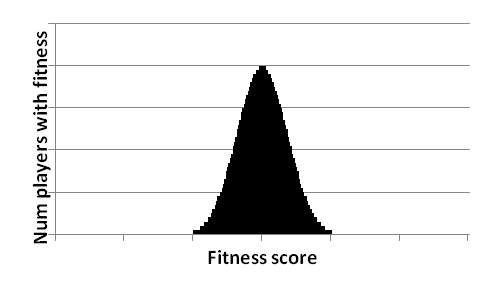
\includegraphics[width=1.0\linewidth]{Figures/binomial.png}
\caption[Binomial Distribution]{The expected fitness distribution for the first
generation of a population that uses a competitive fitness function such as
FINSIH\_ORDER or NUM\_WINS. A peak is expected around the average population
fitness. The distribution is similar to a binomial distribution.}
\label{figure-binomial}
\end{minipage}%
\hspace{0.06\linewidth}%
%%----start of second figure----
\begin{minipage}[t]{0.47\linewidth}
\centering
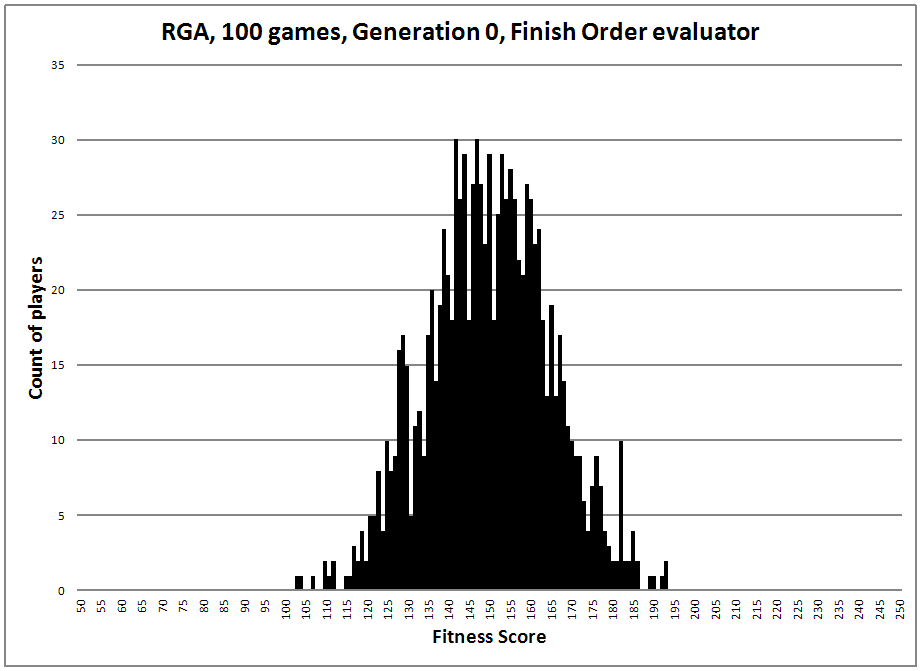
\includegraphics[width=1.0\linewidth]{Figures/RGA_1024_G000_N100_FO.png}
\caption[RGA Finish Order Fitness Distribution, Initial Generation]{RGA
chromosome, size 1024, 100 games per generation, finish order
fitness evaluator, generation 0.}
\label{figure-RGA-G000-N100-FO-initial_fitness}
\end{minipage}
\end{figure}

An example of the fitness distribution for the NUM\_WINS fitness evaluator is
shown in Figure~\ref{figure-RGA-G000-N100-NW-initial_fitness}. The average
fitness for a single game is \(3/4\) or 0.75; for \(n\) games the average
fitness is \(n * 1.5\). The figure shows a binomial shaped distribution which
appears to be centered around the population average of 75.

\begin{figure}
\centering
%%----start of first figure----
\begin{minipage}[t]{0.47\linewidth}
\centering
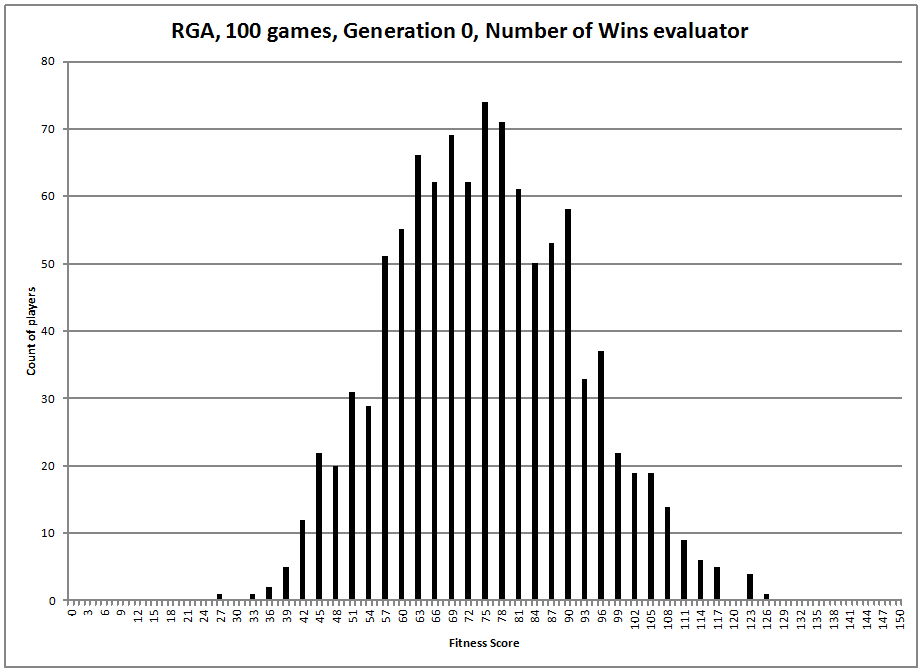
\includegraphics[width=1.0\linewidth]{Figures/RGA_1024_G000_N100_NW.png}
\caption[RGA Num Wins Fitness Distribution, Initial Generation]{RGA chromosome,
size 1024, 100 games per generation, number of wins fitness evaluator,
generation 0.}
\label{figure-RGA-G000-N100-NW-initial_fitness}
\end{minipage}%
\hspace{0.06\linewidth}%
%%----start of second figure----
\begin{minipage}[t]{0.47\linewidth}
\centering
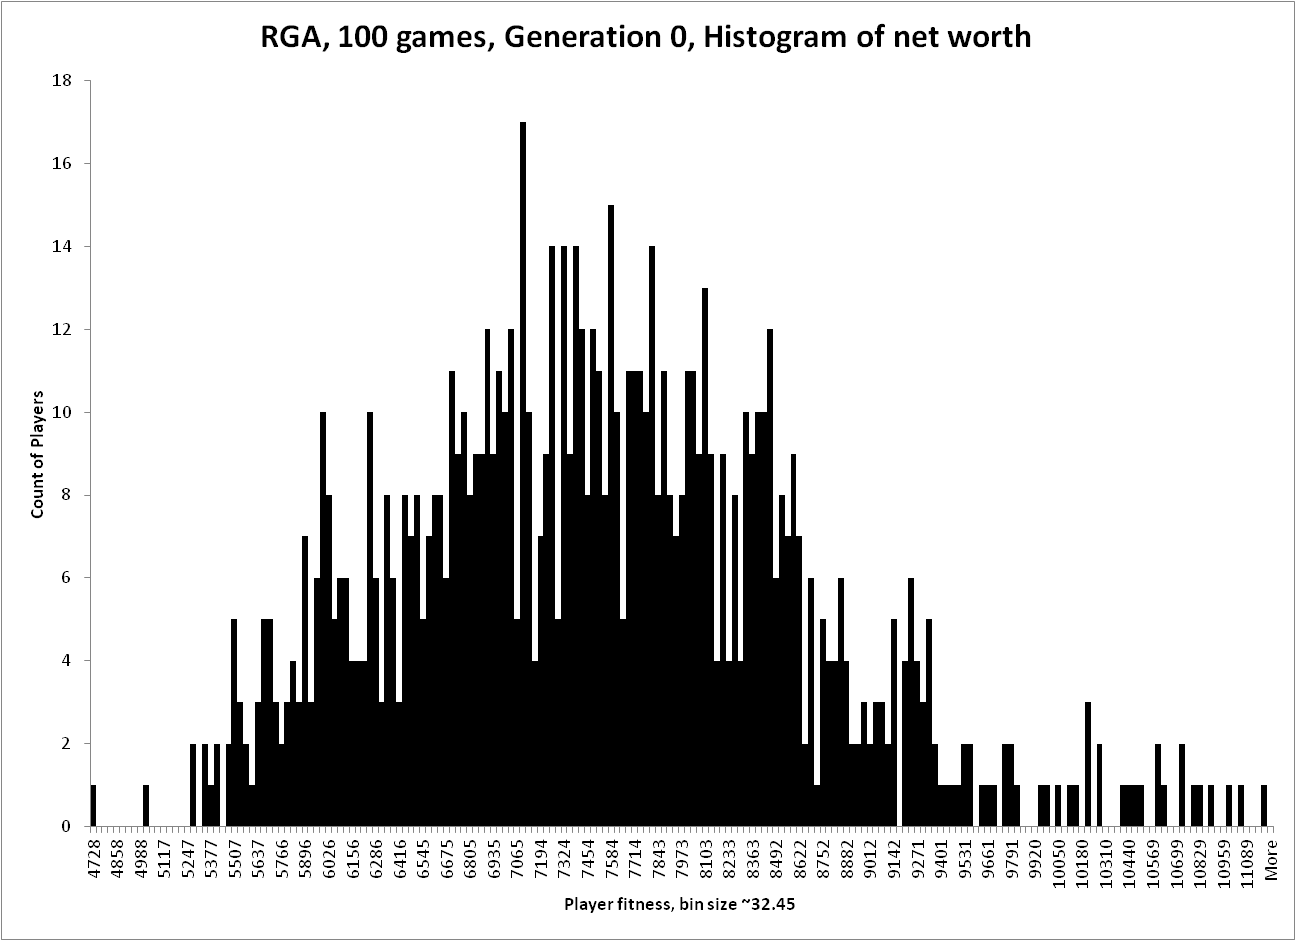
\includegraphics[width=1.0\linewidth]{Figures/RGA_1024_G000_N100_NetW.png}
\caption[Historgram of RGA Net Worth Fitness Distribution, Initial
Generation]{RGA chromosome, size 1024, 100 games per generation, net worth
fitness evaluator, generation 0.}
\label{figure-RGA-G000-N100-NetW-initial_fitness}
\end{minipage}
\\[\intextsep]

\begin{minipage}[t]{0.47\linewidth}
\centering
%%----start of third figure----
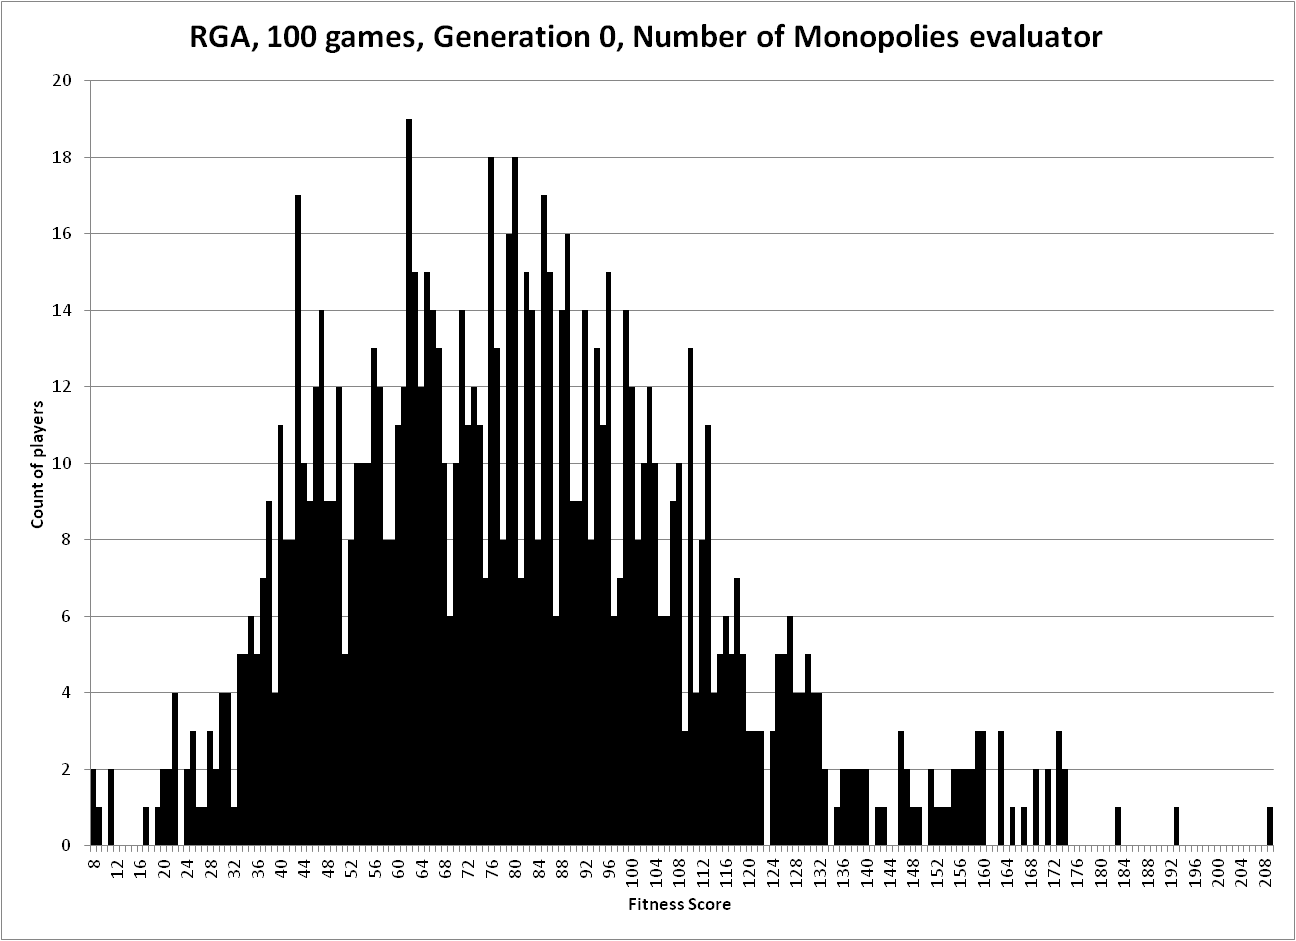
\includegraphics[width=1.0\linewidth]{Figures/RGA_1024_G000_N100_NM.png}
\caption[RGA Num Monopolies Fitness Distribution, Initial Generation]{RGA
chromosome, size 1024, 100 games per generation, number of monopolies
evaluator, generation 0.}
\label{figure-RGA-G000-N100-NM-initial_fitness}
\end{minipage}%
\hspace{0.06\linewidth}%
%%----start of fourth figure----
\begin{minipage}[t]{0.47\linewidth}
\centering
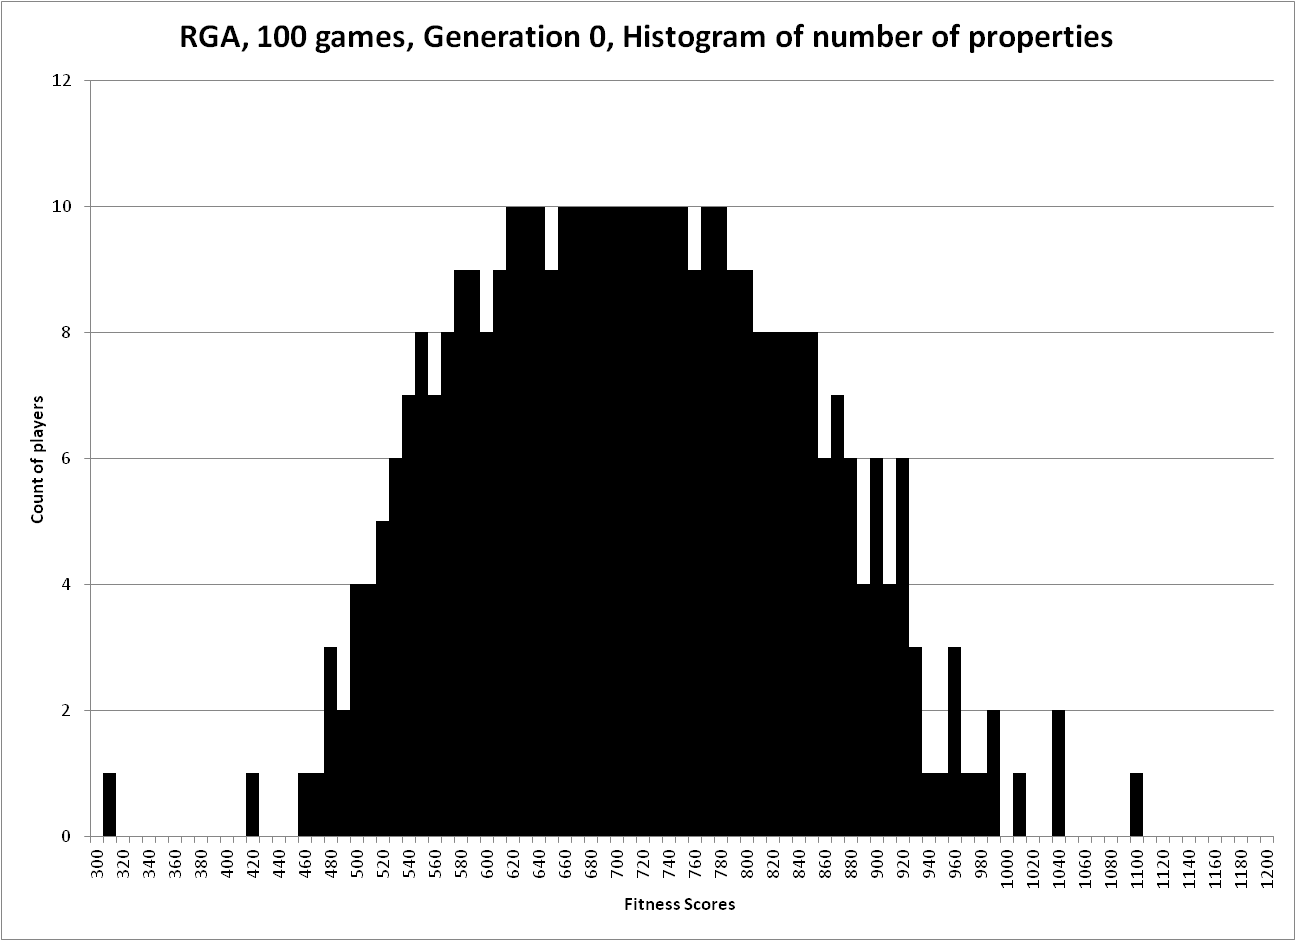
\includegraphics[width=1.0\linewidth]{Figures/RGA_1024_G000_N100_NP.png}
\caption[RGA Num Properties Fitness Distribution, Initial Generation]{RGA
chromosome, size 1024, 100 games per generation, number of properties fitness
evaluator, generation 0.}
\label{figure-RGA-G000-N100-NP-initial_fitness}

\end{minipage}
\end{figure}

Example fitness distributions for the other fitness evaluators are shown in
Figure~\ref{figure-RGA-G000-N100-NetW-initial_fitness},
Figure~\ref{figure-RGA-G000-N100-NM-initial_fitness}, and
Figure~\ref{figure-RGA-G000-N100-NP-initial_fitness}. The distribution for
TOURNAMENT is not shown because it does not follow the same pattern. For
TOURNAMENT, half the population has a score of 0, half of the remainder has a
score of 1, etc., until the final two players have a score of \(log_{2} n-1\).
The TOURNAMENT population will be examined in detail in the validation section.

All of the other populations, regardless of population size, fitness evaluator,
or number of games per generation, show similar results for the initial
generation. These fitness distributions are not surprising. Three of the fitness
evaluators are competitive fitness functions (NUM\_MONOPOLIES and
NUM\_PROPERTIES are not directly competitive, since the player with the most
monopolies or properties is not necessarily the winner of the game). The fact
that the results match previous research into competitive fitness functions
shows that the evolutionary approach we have taken appears to be correct.

\subsection{Results for Subsequent RGA Generations}

As the players get better and the population is more evenly matched, most
players will tend to win half the games they play. As poor players are removed
from the population, the remaining players will tend to be nearer each other in
``ability.'' Thus, the distribution of fitness scores will become much tighter
around the average score, and no single player will be able to dominate the
other players.

For an example of this we look at generation 100 of the RGA-1024-100-FO
population. Figure~\ref{figure-100th_gen_fitness} shows the actual fitness
distribution for this population. The mean remained the same, but the variance
has appeared to decrease. Whereas the fitness scores in generation 0 ranged from
103 to 193, in generation 100 they ranged from 115 to 186. The distribution
around the mean tightened relatively quickly (it can clearly be seen in
generation 100), and then remained fairly constant over the course of the
simulation which was 1000 generations.

\begin{figure}[htp]
\centerline{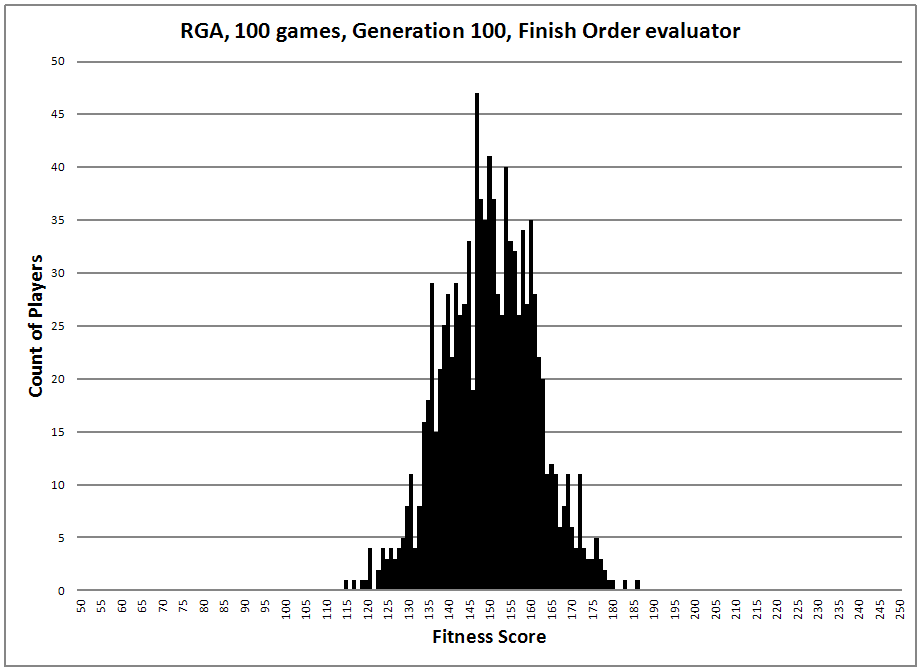
\includegraphics[width=0.75\columnwidth]{Figures/RGA_1024_G100_N100_FO.png}}
\caption[RGA Fitness Distribution, 100th Generation]{RGA chromosome, generation
100, 100 games per generation, finish order fitness evaluator.}
\label{figure-100th_gen_fitness}
\end{figure}

Additional plots of the distribution of fitness scores can be seen in
Figure~\ref{figure-RGA-250th_gen_fitness},
Figure~\ref{figure-RGA-500th_gen_fitness},
Figure~\ref{figure-RGA-750th_gen_fitness}, and
Figure~\ref{figure-RGA-999th_gen_fitness}. Each of these figures shows the
RGA-1024-100-FO population at various points in the evolution process. 

\begin{figure}
\centering
%%----start of first figure----
\begin{minipage}[t]{0.47\linewidth}
\centering
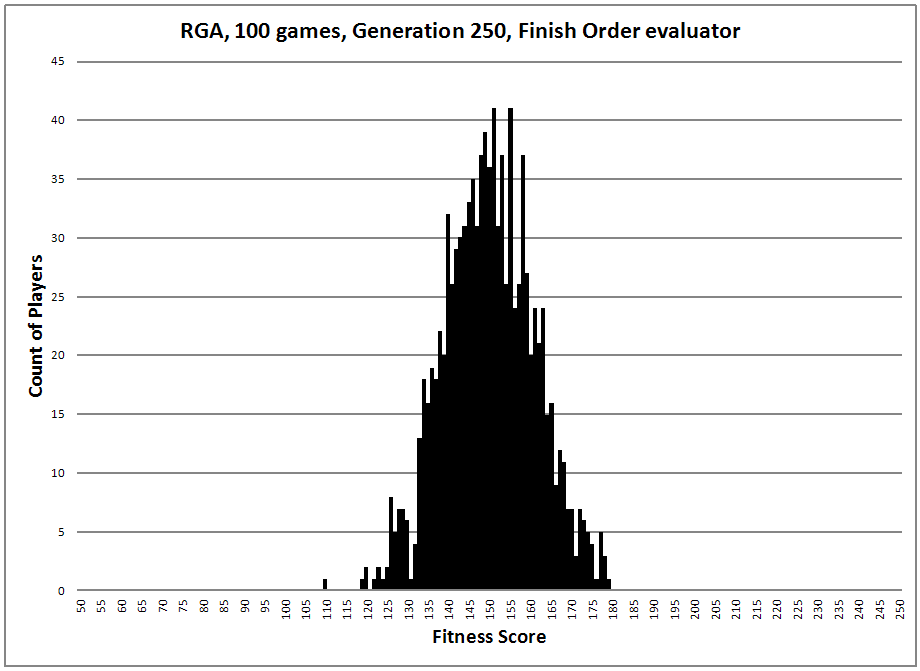
\includegraphics[width=1.0\linewidth]{Figures/RGA_1024_G250_N100_FO.png}
\caption[RGA Fitness Distribution, 250th Generation]{RGA chromosome, size 1024,
100 games per generation, finish order fitness evaluator, generation
250.}
\label{figure-RGA-250th_gen_fitness}
\end{minipage}%
\hspace{0.06\linewidth}%
%%----start of second figure----
\begin{minipage}[t]{0.47\linewidth}
\centering
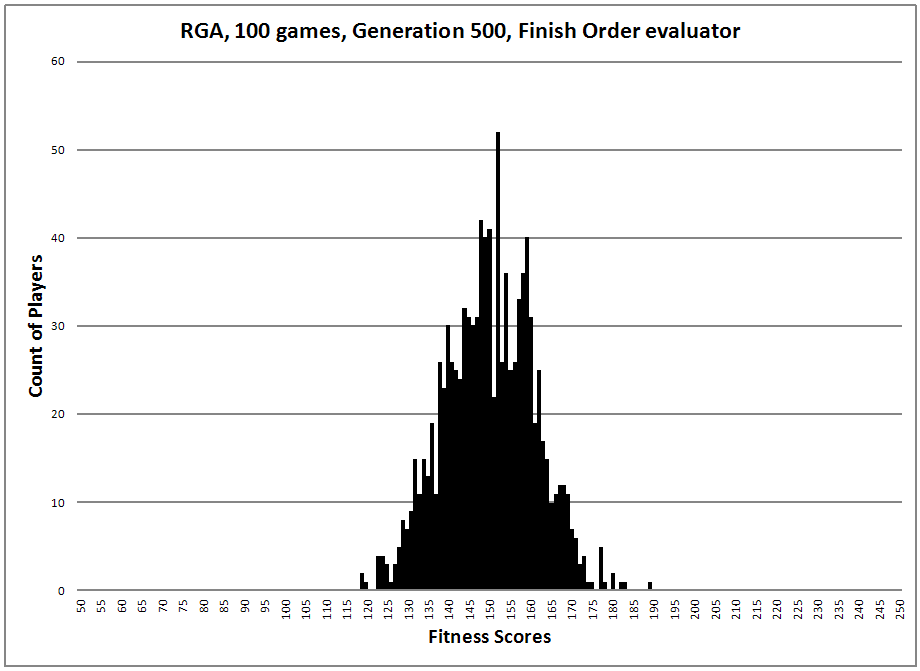
\includegraphics[width=1.0\linewidth]{Figures/RGA_1024_G500_N100_FO.png}
\caption[RGA Fitness Distribution, 500th Generation]{RGA chromosome, size 1024,
100 games per generation, finish order fitness evaluator, generation
500.}
\label{figure-RGA-500th_gen_fitness}
\end{minipage}

\begin{minipage}[t]{0.47\linewidth}
\centering
%%----start of third figure----
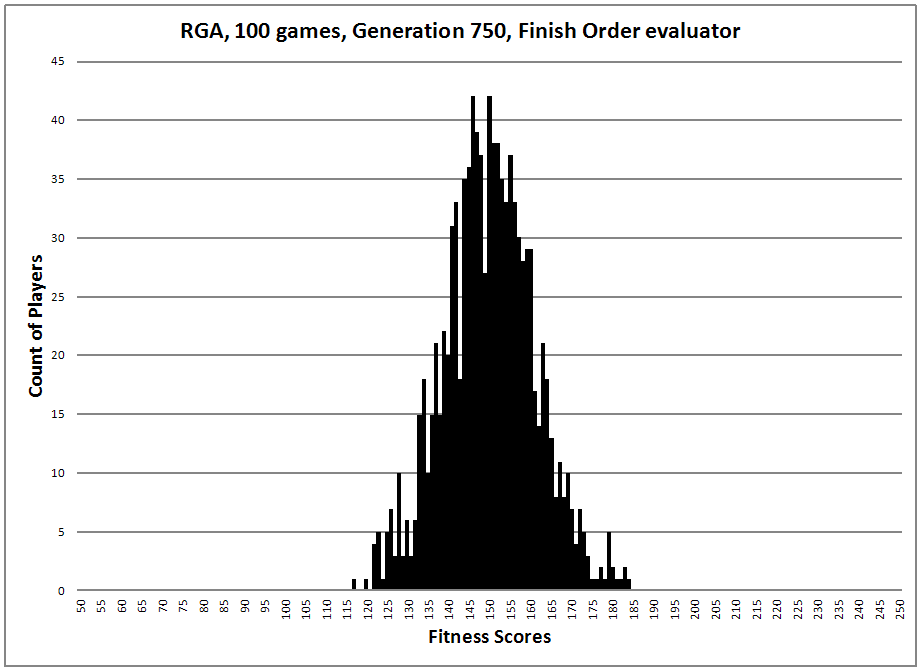
\includegraphics[width=1.0\linewidth]{Figures/RGA_1024_G750_N100_FO.png}
\caption[RGA Fitness Distribution, 750th Generation]{RGA chromosome, size 1024,
100 games per generation, finish order fitness evaluator, generation
750.}
\label{figure-RGA-750th_gen_fitness}
\end{minipage}%
\hspace{0.06\linewidth}%
%%----start of fourth figure----
\begin{minipage}[t]{0.47\linewidth}
\centering
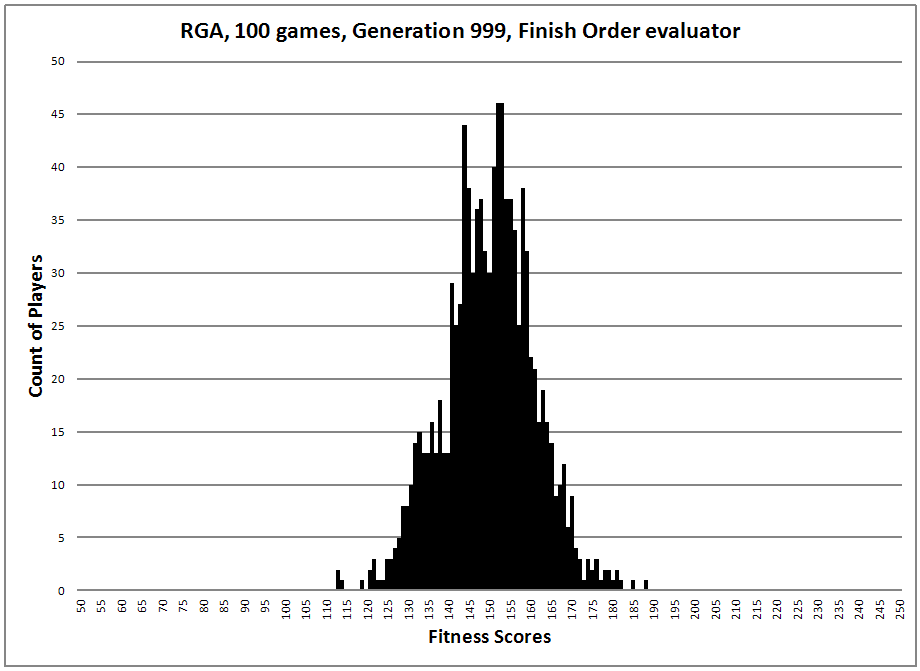
\includegraphics[width=1.0\linewidth]{Figures/RGA_1024_G999_N100_FO.png}
\caption[RGA Fitness Distribution, 999th Generation]{RGA chromosome, size 1024,
100 games per generation, finish order fitness evaluator, generation
999.}
\label{figure-RGA-999th_gen_fitness}
\end{minipage}
\end{figure}

Inspecting Figures~\ref{figure-RGA-250th_gen_fitness} through
\ref{figure-RGA-999th_gen_fitness}, it appears that at some point between the
100th generation and the 250th generation\footnote{Because of the large amount
of data generated by the simulations, data for every generation was not output
by the simulation. Instead fitness data was output and saved for the initial
population, the 100th generation, and every 250th generation. Thus, the point at
which the population average fitness reaches the plateau cannot be calculated.
However, in a coevolutionary environment this is not a problem. A coevolutionary
population can continue to improve even though the fitness appears to plateau.
This will be further discussed later in this Chapter.} that the population
average fitness reaches a plateau. This is also demonstrated by looking at some
of the descriptive statistics for each generation. These are shown in
Table~\ref{table-stats-for-s1024-n100-fo} for the RGA-1024-100-FO population.

\begin{table}[ht]
\begin{center}
\caption[RGA-1024-100-FO statistics]{Descriptive statistics for RGA-1024-100-FO}
\begin{tabular}{ | r || r | r | r | r | r |}
\hline                        
Generation & Min & Max & Average & Variance & Std Dev \\ \hline \hline
0   & 103 & 193 & 150 & 227.43 & 15.08 \\ \hline
100 & 115 & 186 & 150 & 126.81 & 11.26 \\ \hline 
250 & 110 & 179 & 150 & 122.02 & 11.05 \\ \hline
500 & 119 & 189 & 150 & 120.44 & 10.97 \\ \hline
750 & 117 & 184 & 150 & 124.63 & 11.16 \\ \hline
999 & 113 & 188 & 150 & 121.10 & 11.00 \\ \hline
\end{tabular}
\label{table-stats-for-s1024-n100-fo}
\end{center}
\end{table}

In the initial generation, the standard deviation is 15.08, drops to 11.26 by
the 100th generation, and then in the remaining generations (250, 500, 750, and
999) the standard deviation appears to fluctuate around 11.05. We did not
attempt to determine whether this difference in variance between generations is
statistically significant\footnote{To test the hypothesis that the standard
deviations are not equal between generations would require running (in this
example) a population of size 1024 through at least 250 generations, and then
repeating that 250 generation trial enough times to get a statistically
significant sample. Based on the work performed for this research, doing this
for the all of the populations would have taken several weeks of processing
time. It was decided that a better use of resources would be to do a comparative
test between players of different generations and populations.}.

Additional population statistics are in
Table~\ref{table-stats-for-s1024-n100-netw} for the RGA-1024-100-NetW
population, Table~\ref{table-stats-for-s1024-n100-nm} for the RGA-1024-100-NM
population, Table~\ref{table-stats-for-s1024-n100-np} for the RGA-1024-100-NP
population, and Table~\ref{table-stats-for-s1024-n100-nw} for the
RGA-1024-100-NW population.

\begin{table}[ht]
\begin{center}
\caption[RGA-1024-100-NetW statistics]{Descriptive statistics for RGA-1024-100-NetW}
\begin{tabular}{ | r || r | r | r | r | r |}
\hline                        
Generation & Min & Max & Average & Variance & Std Dev \\ \hline \hline
0   & 4728 & 11186 & 7499.99 & 1137919.23 & 1066.73 \\ \hline
250 & 4285 & 10374 & 7499.80 &  649447.67 &  805.88 \\ \hline
500 & 5235 & 10242 & 7500.00 &  665909.43 &  816.03 \\ \hline
750 & 5080 & 10977 & 7500.05 &  723209.97 &  850.42 \\ \hline
999 & 5306 &  9831 & 7499.96 &  649001.83 &  805.61 \\ \hline
\end{tabular}
\label{table-stats-for-s1024-n100-netw}
\end{center}
\end{table}

\begin{table}[ht]
\begin{center}
\caption[RGA-1024-100-NM statistics]{Descriptive statistics for RGA-1024-100-NM}
\begin{tabular}{ | r || r | r | r | r | r |}
\hline                        
Generation & Min & Max & Average & Variance & Std Dev \\ \hline \hline
0   &  8 & 209 &  80.42 & 1014.77 & 31.86 \\ \hline
250 & 37 & 226 & 110.88 &  758.92 & 27.55 \\ \hline 
500 & 43 & 199 & 111.20 &  707.89 & 26.61 \\ \hline
750 & 44 & 199 & 113.97 &  732.09 & 27.06 \\ \hline
999 & 17 & 217 & 116.52 &  734.49 & 27.10 \\ \hline
\end{tabular}
\label{table-stats-for-s1024-n100-nm}
\end{center}
\end{table}

\begin{table}[ht]
\begin{center}
\caption[RGA-1024-100-NP statistics]{Descriptive statistics for RGA-1024-100-NP}
\begin{tabular}{ | r || r | r | r | r | r |}
\hline                        
Generation & Min & Max & Average & Variance & Std Dev \\ \hline \hline
0   & 309 & 1094 & 698.18 &  10271.47 & 101.35 \\ \hline
250 & 504 &  929 & 697.75 &   5322.08 &  72.95 \\ \hline
500 & 478 &  973 & 697.72 &   6126.09 &  78.27 \\ \hline
750 & 462 &  983 & 697.81 &   5928.88 &  77.00 \\ \hline
999 & 438 & 1007 & 697.79 &   6095.32 &  78.07 \\ \hline
\end{tabular}
\label{table-stats-for-s1024-n100-np}
\end{center}
\end{table}

\begin{table}[ht]
\begin{center}
\caption[RGA-1024-100-NW statistics]{Descriptive statistics for RGA-1024-100-NW}
\begin{tabular}{ | r || r | r | r | r | r |}
\hline                        
Generation & Min & Max & Average & Variance & Std Dev \\ \hline \hline
0   & 27 & 126 & 75.00 & 286.43 & 16.92 \\ \hline
250 & 36 & 120 & 75.00 & 155.68 & 12.48 \\ \hline
500 & 30 & 117 & 75.00 & 168.21 & 12.97 \\ \hline
750 & 39 & 120 & 75.00 & 160.36 & 12.66 \\ \hline
999 & 30 & 114 & 75.00 & 173.74 & 13.18 \\ \hline
\end{tabular}
\label{table-stats-for-s1024-n100-nw}
\end{center}
\end{table}

In all of the tables, the average population fitness stays approximately
the same, and the variance in population fitness decreases. Even though it
appears that the variance has plateaued in these examples, players in later
generations can still be improving in fitness. In fact, we show later in this
chapter that players in the last generation are statistically better (i.e., they
win more games) than players in the earliest generations.

This section has focused primarily on the RGA-1024-100 sets of populations. In
general, a similar pattern of statistics is seen in most of the other RGA and
TGA populations that were evolved in this study. Some of the populations,
however, showed weaker, or sometimes conflicting results. A complete set of
tables with that information for the RGA populations can be found in
Appendix~\ref{appendix:rgastats}.

The populations that did not appear to improve over time were the populations
with small population size or small numbers of games per generation. One example
is shown in Table~\ref{tab:6_RGA-0032-007-FO}. In this case, the population
variance gets larger over time, which implies that this population improved
little or none from the first generation to the last. Section~\ref{6_Validation}
provides details on whether the populations did improve or not.

\begin{table}[htbp]
  \centering
  \caption[RGA-0032-007-FO Statistics]{Descriptive Statistics for RGA-0032-007-FO}
    \begin{tabular}{lrrrrrr}
    \toprule
    Population &  Generation & Min    & Max    & Average & Variance & Std Dev \\
    \midrule
    RGA-0032-007-FO & 0      & 4      & 16     & 10.50  & 8.77   & 2.96 \\
    RGA-0032-007-FO & 250    & 4      & 17     & 10.50  & 9.23   & 3.04 \\
    RGA-0032-007-FO & 500    & 5      & 16     & 10.50  & 10.13  & 3.18 \\
    RGA-0032-007-FO & 750    & 2      & 19     & 10.50  & 12.71  & 3.57 \\
    RGA-0032-007-FO & 999    & 5      & 16     & 10.50  & 10.26  & 3.20 \\ 
    \bottomrule
    \end{tabular}
  \label{tab:6_RGA-0032-007-FO}%
\end{table}%

\subsection{Genome Changes Over Time}

We now look at the change in a genome between the initial and final
generations of a population. Using the RGA-1024-100-FO population, part of
the genome for the best player from generation 0 is shown in
Figure~\ref{figure-genome0} and part of the genome for the best player from
generation 999 is shown in Figure~\ref{figure-genome999}. For easier comparison,
the chromosome values from the chart are also shown in
Table~\ref{tab:chromo_compare}.

\begin{figure}[htp]
\centerline{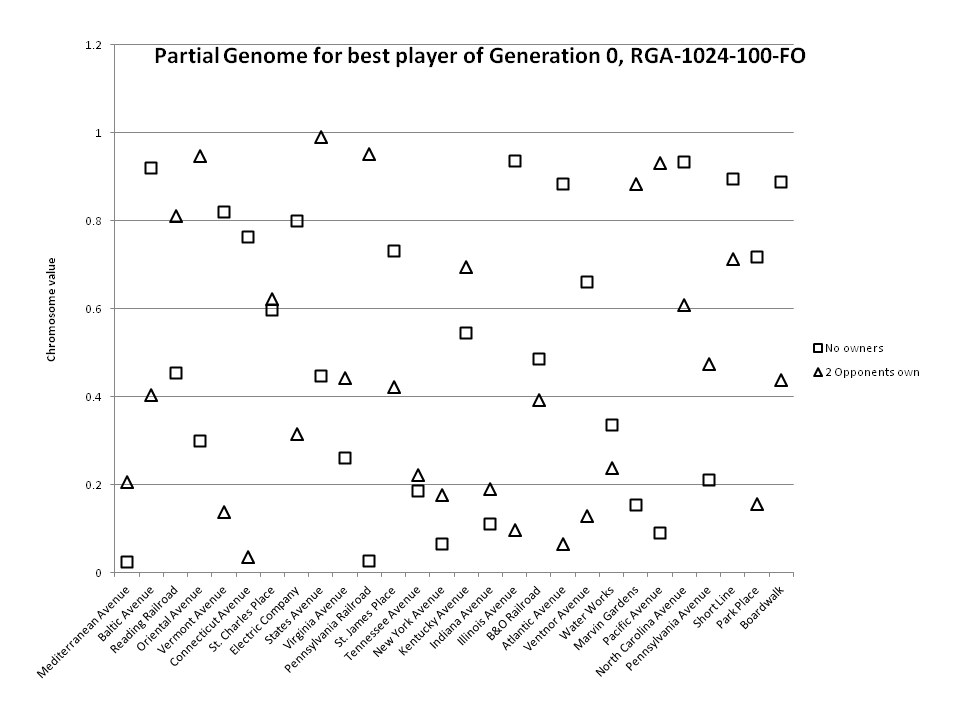
\includegraphics[width=0.75\columnwidth]{Figures/genome000.png}}
\caption[Illustration of Genome, Generation 0]{This chart shows part of the
genome of the fittest player in the first generation of the RGA-1024-100-FO
population. This chart compares the chromosome used when no player owns
any property in the group (represented by the square symbol) against the
chromosome used when two other players own a property in the group (the triangle
symbol).}
\label{figure-genome0}
\end{figure}

\begin{figure}[htp]
\centerline{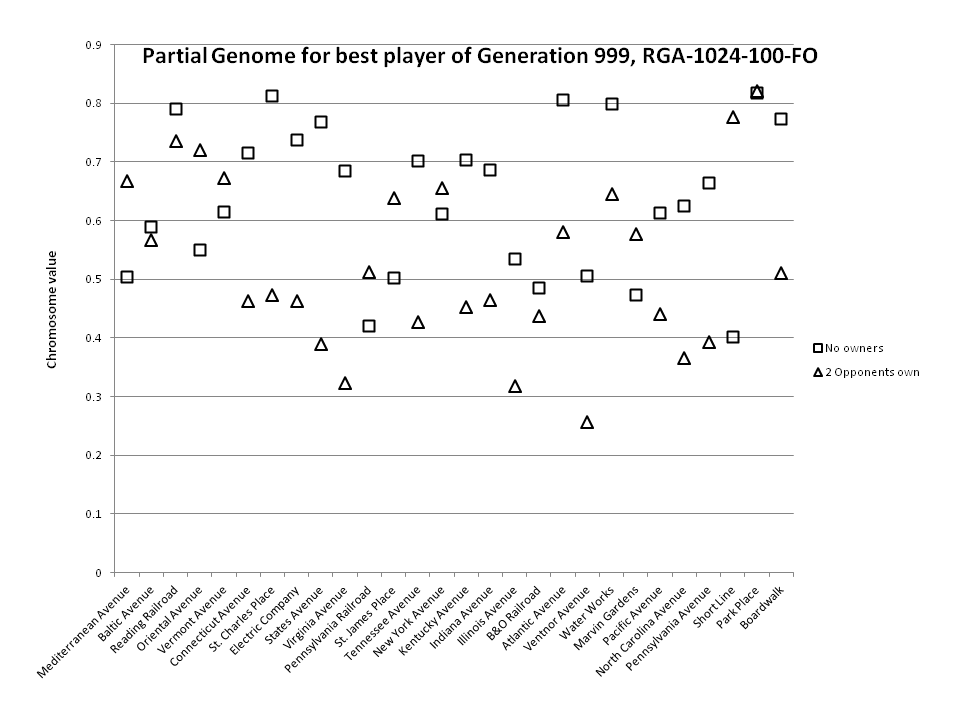
\includegraphics[width=0.75\columnwidth]{Figures/genome999.png}}
\caption[Illustration of Genome, Generation 999]{This chart shows part of the
genome of the fittest player in the last generation of the RGA-1024-100-FO
population. This chart compares the chromosome used when no player owns any
property in the group (the square symbol) against the chromosome used when two
other players own a property in the group (the triangle symbol). These two genes
show agreement with the heuristic strategy: the player is more likely to buy a
property when no one owns a property in the group, and relatively less likely to
buy a property when other players are blocking the group from being
monopolized.}
\label{figure-genome999}
\end{figure}

% Table generated by Excel2LaTeX from sheet 'genome0099 (2)'
\begin{table}[htbp]
  \centering
  \caption[Genome Comparison, Gen 0 vs Gen 999]{Comparison of Best Genomes from Generation 0 and Generation 999}
  \scalebox{0.75}{
    \begin{tabular}{lrrr|rrr}
    \toprule
           & \multicolumn{3}{c|}{Generation 0} & \multicolumn{3}{c}{Generation 999} \\
    \midrule
           & No Owner & 2 Opponents own & Diff   & No Owner & 2 Opponents own & Diff \\
    Mediterranean Avenue & 0.023  & 0.205  & -0.182 & 0.504  & 0.668  & -0.164 \\
    Baltic Avenue & 0.920  & 0.404  & 0.517  & 0.589  & 0.567  & 0.023 \\
    Reading Railroad & 0.454  & 0.810  & -0.356 & 0.790  & 0.736  & 0.054 \\
    Oriental Avenue & 0.300  & 0.947  & -0.648 & 0.550  & 0.721  & -0.171 \\
    Vermont Avenue & 0.821  & 0.138  & 0.683  & 0.614  & 0.673  & -0.059 \\
    Connecticut Avenue & 0.762  & 0.036  & 0.726  & 0.715  & 0.463  & 0.252 \\
    St. Charles Place & 0.598  & 0.622  & -0.024 & 0.812  & 0.473  & 0.339 \\
    Electric Company & 0.799  & 0.314  & 0.484  & 0.737  & 0.463  & 0.274 \\
    States Avenue & 0.448  & 0.991  & -0.543 & 0.768  & 0.389  & 0.379 \\
    Virginia Avenue & 0.260  & 0.442  & -0.182 & 0.685  & 0.323  & 0.362 \\
    Pennsylvania Railroad & 0.027  & 0.952  & -0.925 & 0.421  & 0.512  & -0.091 \\
    St. James Place & 0.730  & 0.423  & 0.308  & 0.502  & 0.639  & -0.137 \\
    Tennessee Avenue & 0.186  & 0.223  & -0.036 & 0.702  & 0.427  & 0.275 \\
    New York Avenue & 0.064  & 0.175  & -0.111 & 0.612  & 0.656  & -0.043 \\
    Kentucky Avenue & 0.544  & 0.694  & -0.150 & 0.704  & 0.452  & 0.252 \\
    Indiana Avenue & 0.110  & 0.189  & -0.080 & 0.686  & 0.465  & 0.221 \\
    Illinois Avenue & 0.936  & 0.096  & 0.840  & 0.536  & 0.319  & 0.217 \\
    B\&O Railroad & 0.487  & 0.391  & 0.095  & 0.485  & 0.437  & 0.048 \\
    Atlantic Avenue & 0.884  & 0.064  & 0.820  & 0.806  & 0.581  & 0.225 \\
    Ventnor Avenue & 0.661  & 0.128  & 0.532  & 0.506  & 0.257  & 0.250 \\
    Water Works & 0.335  & 0.237  & 0.098  & 0.800  & 0.645  & 0.154 \\
    Marvin Gardens & 0.154  & 0.883  & -0.730 & 0.472  & 0.577  & -0.104 \\
    Pacific Avenue & 0.091  & 0.931  & -0.840 & 0.614  & 0.440  & 0.173 \\
    North Carolina Avenue & 0.934  & 0.609  & 0.325  & 0.625  & 0.365  & 0.260 \\
    Pennsylvania Avenue & 0.210  & 0.474  & -0.265 & 0.663  & 0.392  & 0.271 \\
    Short Line & 0.895  & 0.713  & 0.182  & 0.402  & 0.778  & -0.376 \\
    Park Place & 0.718  & 0.155  & 0.563  & 0.818  & 0.822  & -0.004 \\
    Boardwalk & 0.887  & 0.439  & 0.448  & 0.774  & 0.511  & 0.263 \\
    \bottomrule
    \end{tabular}}
  \label{tab:chromo_compare}%
\end{table}%

It can be seen that in general, for the property buying decision, the genome
matches the strategy described previously. The gene values for buying a location
are higher when no player owns one of the properties of a group compared to when
two other players own properties in the group. Although it is not shown in
Figure~\ref{figure-genome999}, the gene values for buying when the player
already owns a property in the group, or when one opponent owns a property in
the group, are generally higher than when two opponents own a property in the
group. A few additional Figures and Tables for some genomes can be found in
Appendix~\ref{appendix:chromos}.

When compared to the strategy list from~\ref{m_gamestrategies}, there might
appear to be an inconsistency in the genome. For example, the strategy says
always buy a property if no one else owns a property in the same group. However,
the greatest gene value in the genome from generation 999 is for Park Place at
0.82. This can easily be explained by the fact that if the player declines a
property with probability \(p_{decline} = 1-p_{buy}\), the probability of
subsequently buying the property is higher. This is because when a player
declines a property, it is then auctioned to any player including the declining
player, and the declining player uses the same chromosome to make the bid
decision independently of the buy decision. So the probability of deciding to
buy a property is
\begin{equation*}
1-(p_{decline} \cdot p_{decline})
\end{equation*}
For example, the probability of a player deciding to buy Park Place with a
chromosome of 0.82 is
\begin{equation*}
1-(0.18 \cdot 0.18) \approx 0.97
\end{equation*}
The probability of actually obtaining the property is slightly lower, however,
since it is dependent on winning the auction.

\subsection{SGA Players} \label{6_SGA}

After evolving the population of RGA Players, the simulation was conducted again
using SGA Players. SGA players are those players with a binary string
chromosome. 

The fitness distribution in the first generation shows the same general
similarity to the binomial distribution (Figure~\ref{figure-sga_gen0}), although
there appears to be a bit of skewness.

\begin{figure}[htp]
\centerline{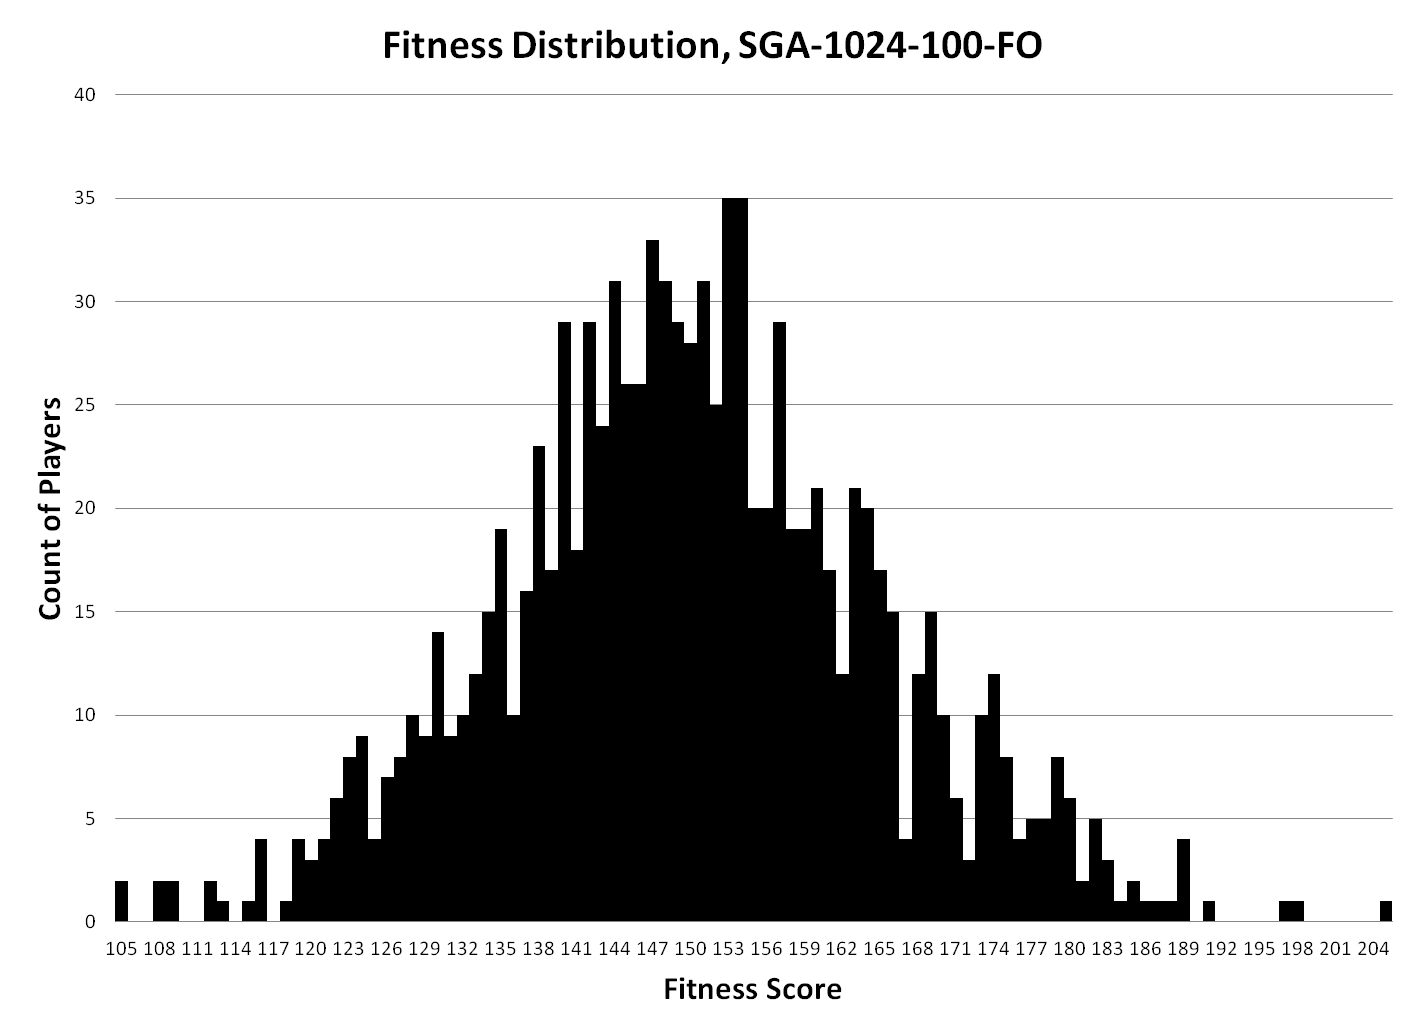
\includegraphics[width=0.75\columnwidth]{Figures/SGA_1024_100_FO_gen0.png}}
\caption[SGA-1024-100-FO Fitness Generation 0]{This figure shows the fitness
distribution for the first generation of the SGA-1024-100-FO population.}
\label{figure-sga_gen0}
\end{figure}

Figure~\ref{figure-sga_gen250} shows the fitness distribution at generation 250
and the skew is definitely present.

\begin{figure}[htp]
\centerline{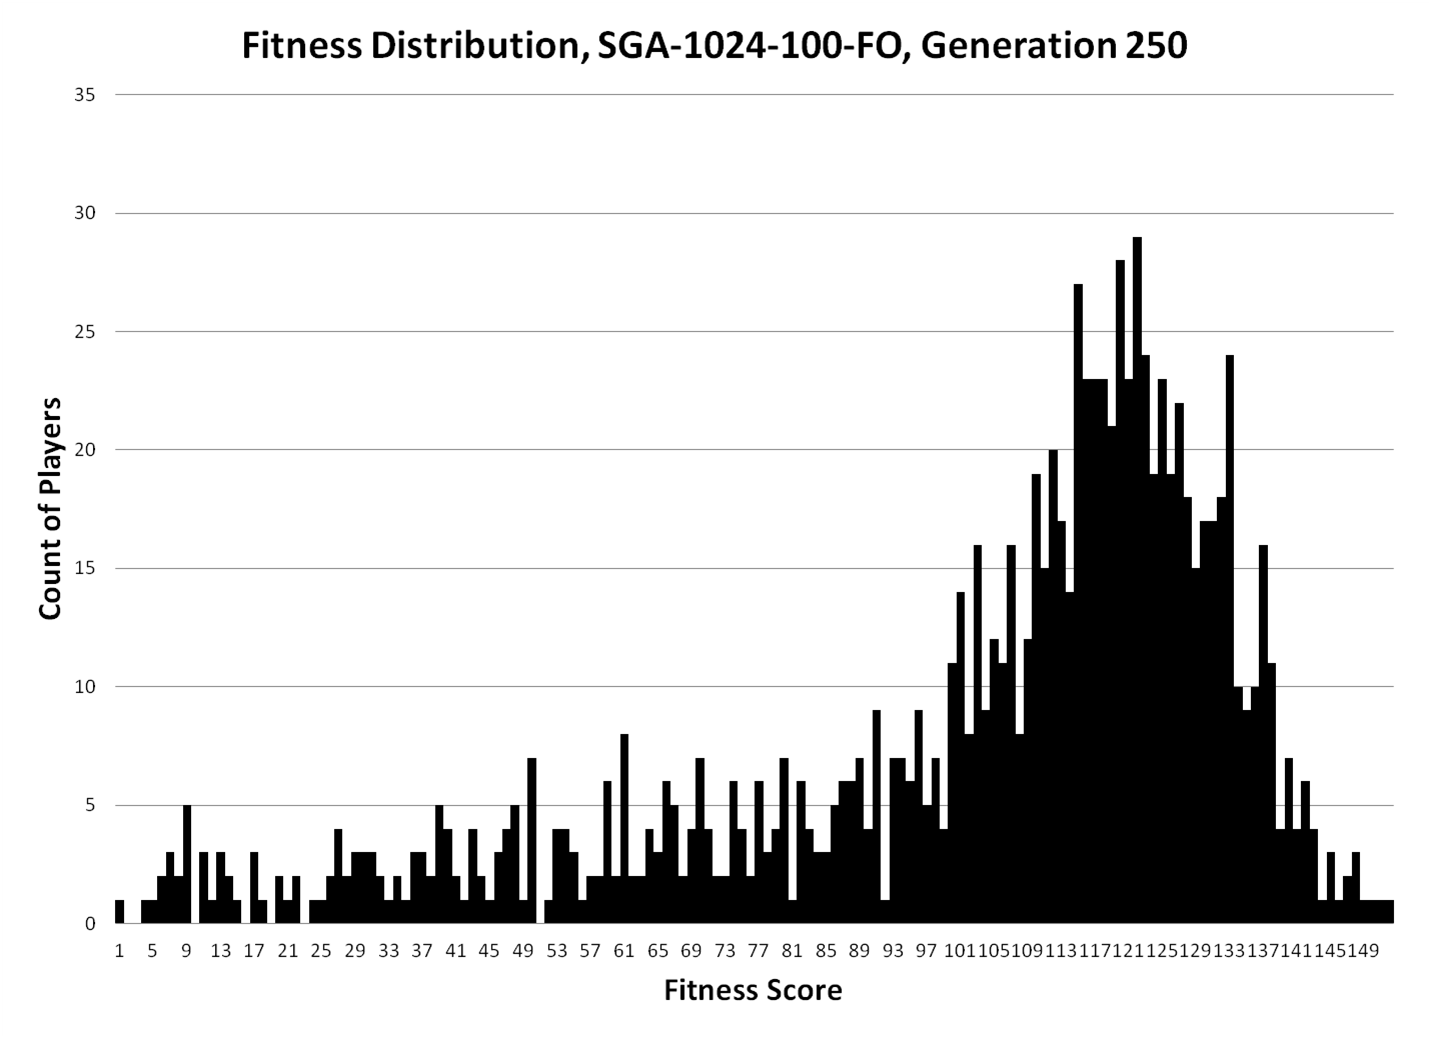
\includegraphics[width=0.75\columnwidth]{Figures/SGA_1024_100_FO_gen250.png}}
\caption[SGA Fitness Generation 289]{This chart shows the fitness
distribution for generation 250 of the SGA-1024-100-FO population.}
\label{figure-sga_gen250}
\end{figure}

Although not shown in this thesis, Generations 500 and 750, for the
SGA-1024-100-FO population, show the same general fitness distribution: a long
tail of low fitness scores, with a peak at higher scores. The fitness
distribution for Generation 999 shows the same pattern and can be seen in
Appendix~\ref{appendix:SGAFitness}. 

Appendix~\ref{appendix:SGAFitness} also contains sample fitness distributions
from other SGA populations. They all show the same pattern. At generation 0,
they are generally symmetric, but sometime prior to generation 250, the
distribution skews so that there is a long tail of low fitness scores, and a
peak of scores higher than the expected average.

At the start of this research, the author thought that the SGA chromosomes would
perform as well as the RGA or TGA chromosomes. Early researchers in genetic
algorithms thought that simple chromosomes would work for most, if not all
problems~\cite{goldberg1989genetic}.

Not only did the fitness distributions show problems, but some initial play
testing of a few of the ``best'' SGA players showed that they performed much
more poorly than the RGA and TGA players, losing in every trial. It was only 
after this that we found the following from Fogel~\cite{fogel1999intelligence}:

\quote{We must also admit that several previous theoretical speculations in 
evolutionary computation have proven to be incorrect. [\ldots] Davis (1991),
Michalewicz (1992), B\"ack and Schwefel (1993), Fogel and Stayton (1994), and
many others, have reported better and faster results in continuous optimization 
problems when using real-valued representations instead of bit strings. \ldots
so the proper conclusion is to use the representation that follows naturally
from the problem and gives you the best insight into discovering improved 
solutions.}

Based on the poor results of the SGA players, and the conclusion that the
chromosome for a problem should not automatically be a bit string, but should be
one best suited to the problem domain, the effort to improve or validate the SGA
chromosome players was no longer pursued as part of this research.

\subsection{TGA Players} \label{6_TGS}

Finally, the same simulation and evolution was conducted using TGA players. The
results for the TGA player were essentially the same as for the RGA player.

The fitness distributions for the initial populations had the same shape as a
binomial distribution, with similar minimums and maximums for the initial
generation as for the RGA chromosomes. Over the 1000 generation simulations, the
fitness distribution converged towards the mean fitness. The minimum, maximum,
mean, and median were essentially the same as the RGA simulation, and the player
genomes were also very similar. This is unsurprising, since the fitness seems to
depend mostly on buying property (in which the RGA and TGA genomes are
identical), and not on getting out of jail which was the difference between the
two genomes.

For this reason, no further validation of the TGA players was pursued. Instead,
the remainder of the study effort focused on validating the RGA players. This
validation is discussed in the next section.

\section{Population Validation} \label{6_Validation}

As with other research that used competitive fitness functions, validations of
the various populations were performed to test if the populations were actually
getting better.

\subsection{Intrapopulation validation}

For every population, the best player in generation 999 was played against
the best player in generations 250, 500, and 750. 100 games were played with the
same set of 4 best players. If the population was actually evolving better
players, we expect that on average, the best player in the last generation will
win more games then the other players; and the best player in the 250th
generation should lose more games on average. 

After 100 games were played, this same trial was repeated 50 times, without
evolution. At the start of validation, 50 games repeated for 100 trials was
chosen to ensure statistically significant results.

Appendix~\ref{appendix:intravalidation} presents the complete set of results for
the RGA-0128 and the RGA-1024 populations. What the tables in the appendix show
is that the populations did improve over time, at least when played against each
other. Table~\ref{tab:validationRGA0128} is an excerpt of the validation results
for the RGA-0128 population (the complete table is in the appendix). 

% Table generated by Excel2LaTeX from sheet 'Finish Order (2)'
\begin{table}[htbp]
  \centering
  \caption{Interpopulation Validation, RGA-0128 partial}
    \begin{tabular}{rrrrrrr}
    \toprule
           &        & \multicolumn{2}{c}{Avg fitness} & \multicolumn{3}{c}{One tailed t test} \\
    \midrule
    Number of games per generation in original population & original fitness evaluator & \multicolumn{1}{c}{Generation 250} & \multicolumn{1}{c}{Generation 500} & \multicolumn{1}{c}{t test G250 vs G500} & \multicolumn{1}{c}{t test G500 vs G750} & \multicolumn{1}{c}{t test G750 vs G999} \\
    \multicolumn{1}{l}{\multirow{5}[10]{*}{100}} & finish order & 1389.42 & 1489.52 & 0.00   & 0.00   & 0.00 \\
    \multicolumn{1}{l}{} & net worth & 1426.96 & 1472.62 & 0.00   & 0.00   & 0.00 \\
    \multicolumn{1}{l}{} & num monop & 1464.06 & 1494.22 & 0.00   & 0.15   & 0.00 \\
    \multicolumn{1}{l}{} & num props & 1438.08 & 1487.34 & 0.00   & 0.00   & 0.00 \\
    \multicolumn{1}{l}{} & num wins & 1418.00 & 1493.70 & 0.00   & 0.00   & 0.04 \\
    \bottomrule
    \end{tabular}%
  \label{tab:validationRGA0128}%
\end{table}%

Each row represents a single population. The first row, for example, is the
RGA-0128-100-FO population. The best player from generations 250, 500, 750, and
999 were competed against each other. In these trials, the fitness of each
player is evaluated using finish order evaluator. The score in the average
fitness column is the average fitness scores for that player over 50 trials of
100 games per trial. To evaluate whether players in later generations were
better than players in earlier generations, a one-tailed Student's t-test was
performed with H_{0} that the average fitness is the same for each generation.
In most cases, the null hypothesis is rejected, indicating that the average
fitness scores are different. Since average fitness increases over time, the
one-tailed t-test says that not only are the fitness scores different, the
average fitness is increasing over time.

The table above shows 3 of the tests: generation 250 compared to generation 500,
500 to 750, and 750 to 999. At almost any significance level, the results
indicate that almost every later generation is better than every earlier
generation. One of the exceptions in the table above is for the NUM\_MONOPOLIES
evaluator in the comparison of generation 500 to generation 750. For that test
we accept the null hypothesis and must conclude that the players from those two
generations have the same ability.

However, looking at all the results in Appendix~\ref{appendix:intravalidation},
we reject the null hypothesis for most of the tests.

Where we tend to accept the null hypothesis most often is for populations with
a small number of games per generation, and for populations that are temporally
close to each other. For example, looking at the RGA-0128 table in the Appendix,
when the number of games per generation is 7, The null hypothesis is accepted
14 out of 25 trials at the 0.05 significance level. Looking at the same table,
the null hypothesis is accepted most often when comparing Generation 500 to 750
(accepted 9 times), and when comparing Generation 750 to 999 (accepted 8 times). 

The conclusion from this set of experiments is that better players evolved in
larger populations that played large numbers of games per generation.

\subsection{Interpopulation validation}

Next, the best players from the last generation of similar populations that used
different fitness evaluators were played against each other. This was done to
see which, if any, fitness evaluator produced better players. Because of the
highly random nature of the game and based on the previous work comparing
competitive fitness functions, we expected that the TOURNAMENT fitness evaluator
would produce less fit players than at least some of the other fitness
evaluators.

RESULTS PENDING

\section{Human versus RGA competition}

Based on the results of the evolutionary phase of this study, a set of RGA
players was selected and competed against human players to validate the
evolutionary results. The results of these competitions is presented here.

The intra- and iter-population analysis showed that the best results came from
populations with high population size, many games per generation, and from the
latest generations of the evolution. For those reasons, players for this
validation were selected from the RGA-1024-100-FO population. 

\subsection{Human versus computer validation I}

The first competition was conducted after implementing the trading algorithm
proposed by Yasumura, et al, in ``Negotiation strategy of agents in the MONOPOLY
game~\cite{Yasumura2001Negotiate}''. 

The algorithm evaluates the ownership situation of the properties being traded,
and then sums various combinations of gains based on that situation. For
example, if a trade would lead to a Monopoly, the algorithm computes the sum of
3 times the expected long-term gain, and the expected mid- and short-term
gains\footnote{Mid-term is defined as the gain or loss after one trip around the
board; short-term is defined as the gain or loss after one dice roll.}, and
adjusts that by a factor \(\omega\). It then subtracts the short- and mid-term
losses, which are adjusted by the factor \(1-\omega\). When the player would be
the only owner of only one property in a group, then a different combination of
gains is summed (long-term gain is less important in this case).

When \(\omega\) is close to 1, the player values gains and completely ignores
losses; alternately, when \(\omega\) is close to 0, the player is more sensitive
to losses. The algorithm results in a value \(U\) which is the gain (or loss)
from the trade.

If the value \(U\) exceeds some threshold, the player proposes the trade, or
accepts the trade. In their paper, Yasumura, et al, claimed that when their
algorithm was compared to the game play of human experts, the algorithm matched
the humans when gains and losses were balanced \(\omega \approx 0.5\)), and when
the threshold was relatively low (approximately 100).

So the algorithm was implemented with those parameters: \(\omega = 0.5\)), and 
threshold of 100.

The best 4 players from generations 250, 500, 750, and 999 of the 
RGA-1024-100-FO populations were selected. They then competed in a Monopoly game
player against a single human player. For each game, the game chose 3 RGA 
opponents at random. So usually the human player was playing against a mix of
players from the 4 generations. This was done to perform a secondary validation
of the fact that players from later generation should be better than players
from earlier generations. If that was the case as proved in the intra-population
validation, then regardless of how the RGA players played against the human 
players in aggregate, the players from generation 999 should still do better 
than the players from generation 250.

The results of this initial human versus computer validation are shown in 
Table~\ref{tab:human_rga_I}.

      % Table generated by Excel2LaTeX from sheet 'Pivot table'
      \begin{table}[htbp]
        \centering
        \caption[Human versus RGA results, initial]{Results of Human versus RGA
        player competitions, with initial trading algorithm}
          \begin{tabular}{r|rrr}
          \toprule
                 & Results &        &  \\
          \midrule
          Players & Average finish & Average networth & Count of games
          \\ \\
          \multicolumn{1}{l|}{gen250} & 2.8    & 1170.1 & 85.0 \\
          \hline
          \multicolumn{1}{l|}{player0040.dat} & 2.6    & 2207.0 & 26.0 \\
          \multicolumn{1}{l|}{player0191.dat} & 2.5    & 765.2  & 15.0 \\
          \multicolumn{1}{l|}{player0478.dat} & 3.0    & 416.2  & 22.0 \\
          \multicolumn{1}{l|}{player0752.dat} & 3.0    & 974.6  & 22.0 \\ \\
          \multicolumn{1}{l|}{gen500} & 2.8    & 1137.4 & 78.0 \\
          \hline
          \multicolumn{1}{l|}{player0028.dat} & 2.8    & 902.8  & 25.0 \\
          \multicolumn{1}{l|}{player0445.dat} & 2.9    & 1291.4 & 21.0 \\
          \multicolumn{1}{l|}{player0913.dat} & 2.7    & 404.6  & 19.0 \\
          \multicolumn{1}{l|}{player0923.dat} & 2.8    & 2410.8 & 13.0 \\ \\
          \multicolumn{1}{l|}{gen750} & 2.7    & 1367.1 & 92.0 \\
          \hline
          \multicolumn{1}{l|}{player0453.dat} & 2.9    & 332.1  & 28.0 \\
          \multicolumn{1}{l|}{player0474.dat} & 2.6    & 1910.8 & 28.0 \\
          \multicolumn{1}{l|}{player0524.dat} & 2.6    & 1195.1 & 18.0 \\
          \multicolumn{1}{l|}{player0750.dat} & 2.6    & 2303.2 & 18.0 \\ \\
          \multicolumn{1}{l|}{gen999} & 2.9    & 954.7  & 72.0 \\
          \hline
          \multicolumn{1}{l|}{player0101.dat} & 3.0    & 762.1  & 18.0 \\
          \multicolumn{1}{l|}{player0423.dat} & 3.1    & 730.9  & 14.0 \\
          \multicolumn{1}{l|}{player0667.dat} & 2.7    & 1645.2 & 13.0 \\
          \multicolumn{1}{l|}{player0928.dat} & 3.0    & 866.6  & 27.0 \\ \\
          \multicolumn{1}{l|}{human} & 1.6    & 7484.0 & 109.0 \\
          \hline
          \multicolumn{1}{l|}{A} & 1.6    & 7926.6 & 19.0 \\
          \multicolumn{1}{l|}{B} & 1.3    & 9141.6 & 24.0 \\
          \multicolumn{1}{l|}{C} & 2.3    & 5443.4 & 8.0 \\
          \multicolumn{1}{l|}{E} & 1.9    & 6311.3 & 12.0 \\
          \multicolumn{1}{l|}{G} & 2.3    & 3030.3 & 3.0 \\
          \multicolumn{1}{l|}{H} & 1.6    & 7371.2 & 13.0 \\
          \multicolumn{1}{l|}{S} & 1.5    & 7644.7 & 23.0 \\
          \multicolumn{1}{l|}{K} & 1.0    & 11473.0 & 3.0 \\
          \multicolumn{1}{l|}{V} & 2.5    & 5654.5 & 2.0 \\
          \multicolumn{1}{l|}{L} & 2.0    & 0.0    & 1.0 \\
          \multicolumn{1}{l|}{T} & 3.0    & 0.0    & 1.0 \\ \\
          \multicolumn{1}{l|}{Grand Total} & 2.5    & 2748.7 & 436.0 \\
          \bottomrule
          \end{tabular}%
        \label{tab:human_rga_I}%
      \end{table}%

Clearly, for this set of competitions, the human players greatly out-played the
RGA players. The average score for the human players was noticeably better than
the average score for any generation of RGA players. The average net worth of
every human player (except for two outliers who only played a single game and
lost) was higher than the average net worth of every computer player.

After analyzing the results and conducting interviews with several of the human
players, the following was noted:

\begin{itemize} 
  \item {The RGA players tended to propose a lot of trades, as often
  as once per turn.}
  \item {The human players who participated in this competition rarely proposed
  trades. Part of that is because it was easier to let the RGA player make a 
  proposal, and accept or reject that. Another reason is that the trade 
  threshold for the human players was much higher than 100 threshold of the RGA 
  players.}
  \item {These proposed trades, while they may have exceeded the profit 
  threshold for the player, were often obviously bad trades for the RGA player 
  (for example, trading a property that resulted in a monopoly for the human, 
  but no monopoly for the RGA player).}
  \item {Although being able to buy property is useful, it is just as important
  in this game to be able to trade well.}
\end{itemize}

 \subsection{Human versus computer validation II}
 
 Based on the results of the first human versus computer competition, the traindg
 algorithm was updated by raising the threshold for accepting or proposing a trade
 to either 200 or 400 potential gain, and changing \(\omega\) to be either
 0.65, 0.80, or 0.95.
 
 Human volunteers then played the game again. Preliminary results show some 
 improvement in trading behavior: the RGA players propose less trades, and the
 trades the do propose are more sensible than they were previously.
 
 However this did not improve their game play enough. Preliminary results show 
 the human players winning approximately 39 games to the RGA players' 11 wins.
 
 Final results a re pending.
 
 \section{Summary}
 
 Although it appears that evolutionary computing can be used to learn when to
 make property buying decisions in the game of Monopoly, the RGA players were
 hampered in this experiment by having a trading algorithm that sometimes
 resulted in making bad trades which led to losses against human players. That
 is probably partly due to the trading algorithm and partly due to
 implementation decisions made when the algorithm was coded.
 